\documentclass[12pt]{hsrthesis}
\makeindex
\makeglossaries
%add new glossaryentries here...

\newglossaryentry{RQ}{
	name=RQ,
	description={RQ (Redis Queue) ist ist eine einfache Library für Python um Jobs in Redis einzureihen},
	first={RQ}
}

\newglossaryentry{Mapquest}{
	name=Mapquest,
	description={Mapquest ist eine API für OpenStreetMap Daten},
	first={Mapquest}
}

\newglossaryentry{Maptiler}{
	name=Maptiler,
	description={Maptiler bietet ein Python Skript zur Umrechnung von Koordinaten zu Tiles},
	first={Maptiler}
}

\newglossaryentry{Quadkeys}{
	name=Quadkeys,
	description={Quadkeys werden von Bing Maps für die Referenzierung zu ihren Tiles verwendet},
	first={Quadkeys}
}

\newglossaryentry{CircleCI}{
	name=CircleCI,
	description={CircleCI ist ein Tool für Continuous Integration und Deployment},
	first={CircleCI}
}

\newglossaryentry{Jira}{
	name=Jira,
	description={Jira ist eine webbasierte Anwendung für  Projektmanagement},
	first={Jira}
}

\newglossaryentry{PyCharm}{
	name=PyCharm,
	description={PyCharm ist eine IDE von JetBrains für Python},
	first={PyCharm}
}

\newglossaryentry{GitHub}{
	name=GitHub,
	description={GitHub ist ein webbasierter Dienst für Software-Entwicklungsprojekte},
	first={GitHub}
}

\newglossaryentry{Git}{
	name=Git,
	description={Git ist ein Versionsverwaltungssystem},
	first={Git}
}

\newglossaryentry{OpenStreetMap}{
	name=OpenStreetMap,
	description={Online Karten Anwendung wie Google Maps},
	first={OpenStreetMap}
}

\newglossaryentry{Orthofotos}{
	name=Orthofotos,
	description={Luftbilder, umgangssprachlich Satellitenbilder},
	first={Orthofotos}
}

\newglossaryentry{Convolutional Neural Network}{
	name=Convolutional Neural Network,
	description={Neuronales Netz speziell für Bilderkennung},
	first={Convolutional Neural Network}
}

\newglossaryentry{Convnet}{
	name=Convnet,
	description={Abkürzung für Convolutional Neural Network},
	first={Convnet}
}

\newglossaryentry{Deep Learning}{
	name=Deep Learning,
	description={Marketingbegriff für tiefe Neuronale Netze},
	first={Deep Learning}
}

\newglossaryentry{MapRoulette}{
	name=MapRoulette,
	description={Online Crowdsourcing-System zur spielerischen Überprüfung von Daten für OpenStreetMap},
	first={MapRoulette}
}

\newglossaryentry{To-Fix}{
	name=To-Fix,
	description={Online Crowdsourcing-System zur spielerischen Überprüfung von Daten},
	first={To-Fix}
}

\newglossaryentry{Docker}{
	name=Docker,
	description={Leichtgewichtige Virtualisierung},
	first={Docker}
}

\newglossaryentry{Confusion Matrix}{
	name=Confusion Matrix,
	description={Wahrheitsmatrix, Methode zur Bewertung von Klassifizieren},
	first={Confusion Matrix}
}

\newglossaryentry{Haar Feature-based Cascade Classifier}{
	name=Haar Feature-based Cascade Classifier,
	description={Bilderklassifizierer aus OpenCV},
	first={Haar Feature-based Cascade Classifier}
}

\newglossaryentry{Scale-invariant Feature Transform}{
	name=Scale-invariant Feature Transform,
	description={Bildwiedererkenner aus OpenCV},
	first={Scale-invariant Feature Transform}
}

\newglossaryentry{Tile}{
	name=Tile,
	description={Quadratisches Bild mit Karteninhalt, Kachel},
	first={Tile}
}

\newglossaryentry{Bounding Box}{
	name=Bounding Box,
	description={Eine Fläche, welche durch zwei Längengrade und zwei Breitengrade definiert ist},
	first={Bounding Box}
}

\newglossaryentry{Keras}{
	name=Keras,
	description={Python Bibliothek zum Training und der Verwendung von Neuronalen Netzen},
	first={Keras}
}

\newglossaryentry{OpenCV}{
	name=OpenCV,
	description={C++ Bibliothek zur Verarbeitung von Bildern und Videos},
	first={OpenCV}
}

\newglossaryentry{Inputbild}{
	name=Inputbild,
	description={RGB Bild mit der Grösse 50 x 50 Pixel, welches als Input eines Convnet dient},
	first={Inputbild}
}

\newglossaryentry{QuadTree}{
	name=QuadTree,
	description={Format zur Identifizierung von Tiles},
	first={QuadTree}
}



\raggedbottom %http://blog.emeidi.com/2009/03/07/damit-latex-paragraphen-nicht-vertikal-auf-die-seite-verteilt/
%Anhang
%%%%%%%%%%%%%%%%%%%%%%%%%%%%%%
\makeatletter
\g@addto@macro\appendix{%
  \cleardoublepage
  \hypertarget{appendixstart}{}%
  \addtocontents{toc}{
    \protect\contentsline{chapter}{\protect\hyperlink{appendixstart}{Anhang}}{}{}%
}%
}

\makeatother

\begin{document}
\newcommand{\thesistitle}{strongMan}
\newcommand{\thesisauthora}{Bühler Severin}
\newcommand{\thesisauthorb}{Kurath Samuel}
\newcommand{\thesisauthorc}{}
\newcommand{\professor}{Prof. Dr. Andreas Steffen}
\newcommand{\thesistype}{Bachelorarbeit}
\newcommand{\departement}{Abteilung Informatik}
\newcommand{\school}{HSR Hochschule für Technik Rapperswil}
\newcommand{\term}{Frühjahrssemester 2016}
\newcommand{\thedate}{18. Juni 2016}
\newcommand{\timeperiode}{22.02.2016 - 18.06.2016}


\setlength{\oddsidemargin}{20mm}
\maketitle
\setlength{\oddsidemargin}{20mm}

\newpage
\mbox{}\\
\newpage
\section{Abstract}
Die VPN Applikation ist weltweit stark verbreitet, nun soll es möglich sein die Konfiguration per graphischen Interface zu vereinfachen.\\


Weitere Informationen: \url{https://github.com/strongswan/}\\ \\ \\ \\


\section{Management Summary}
\subsection*{Ausgangslage}
Management per UI.

\subsection*{Vorgehen}
Erarbeitung der Lösung


\subsection*{Ergebnisse}
BA


\subsection*{Ausblick}
Erweitern
\newpage

% List of Contents
%%%%%%%%%%%%%%%%%%%%%%%%%%%%
\tableofcontents
\newpage
\listoffigures
\newpage
\listoftables
\newpage
\listofdecision

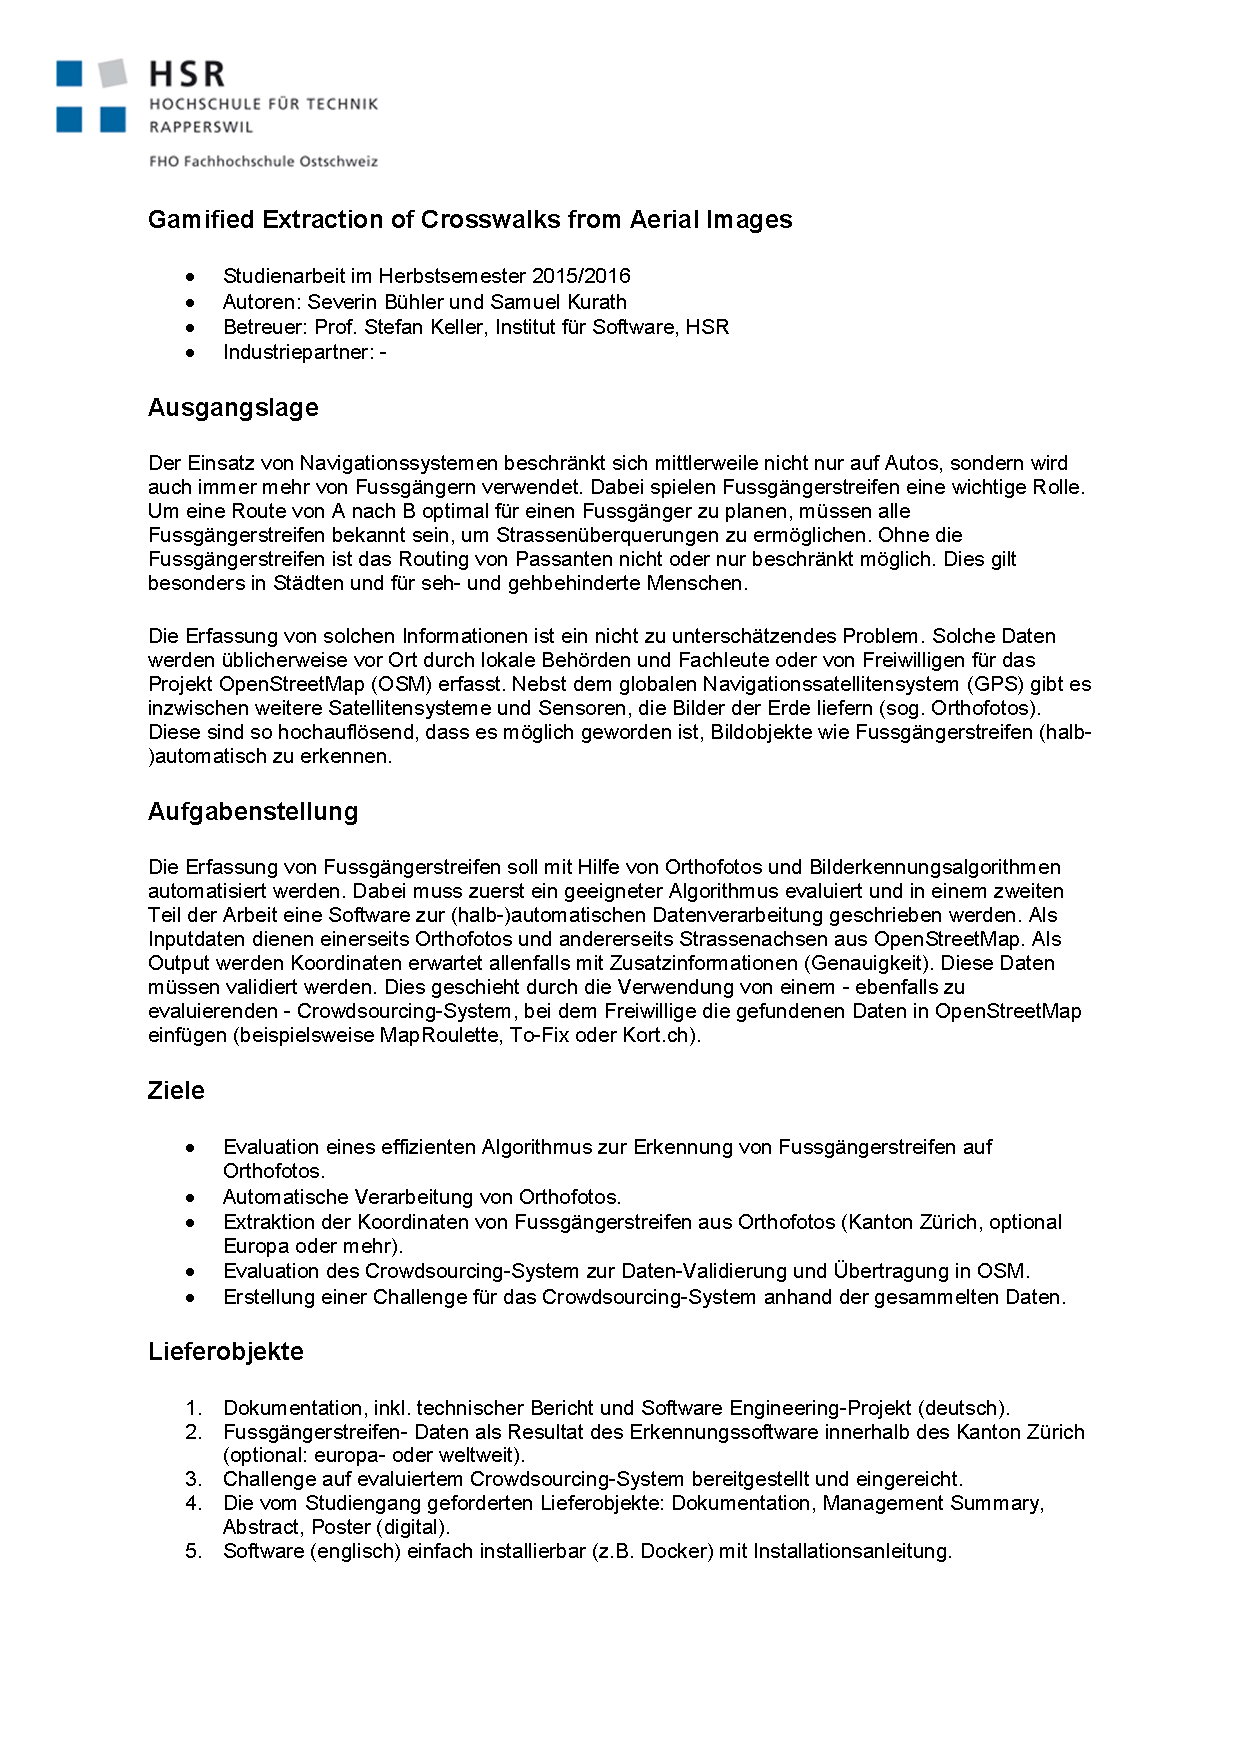
\includepdf[pages=-,offset=75 -75,frame,scale=.75,pagecommand={\section{Aufgabenstellung}}]{pdfs/aufgabenstellung1.pdf}
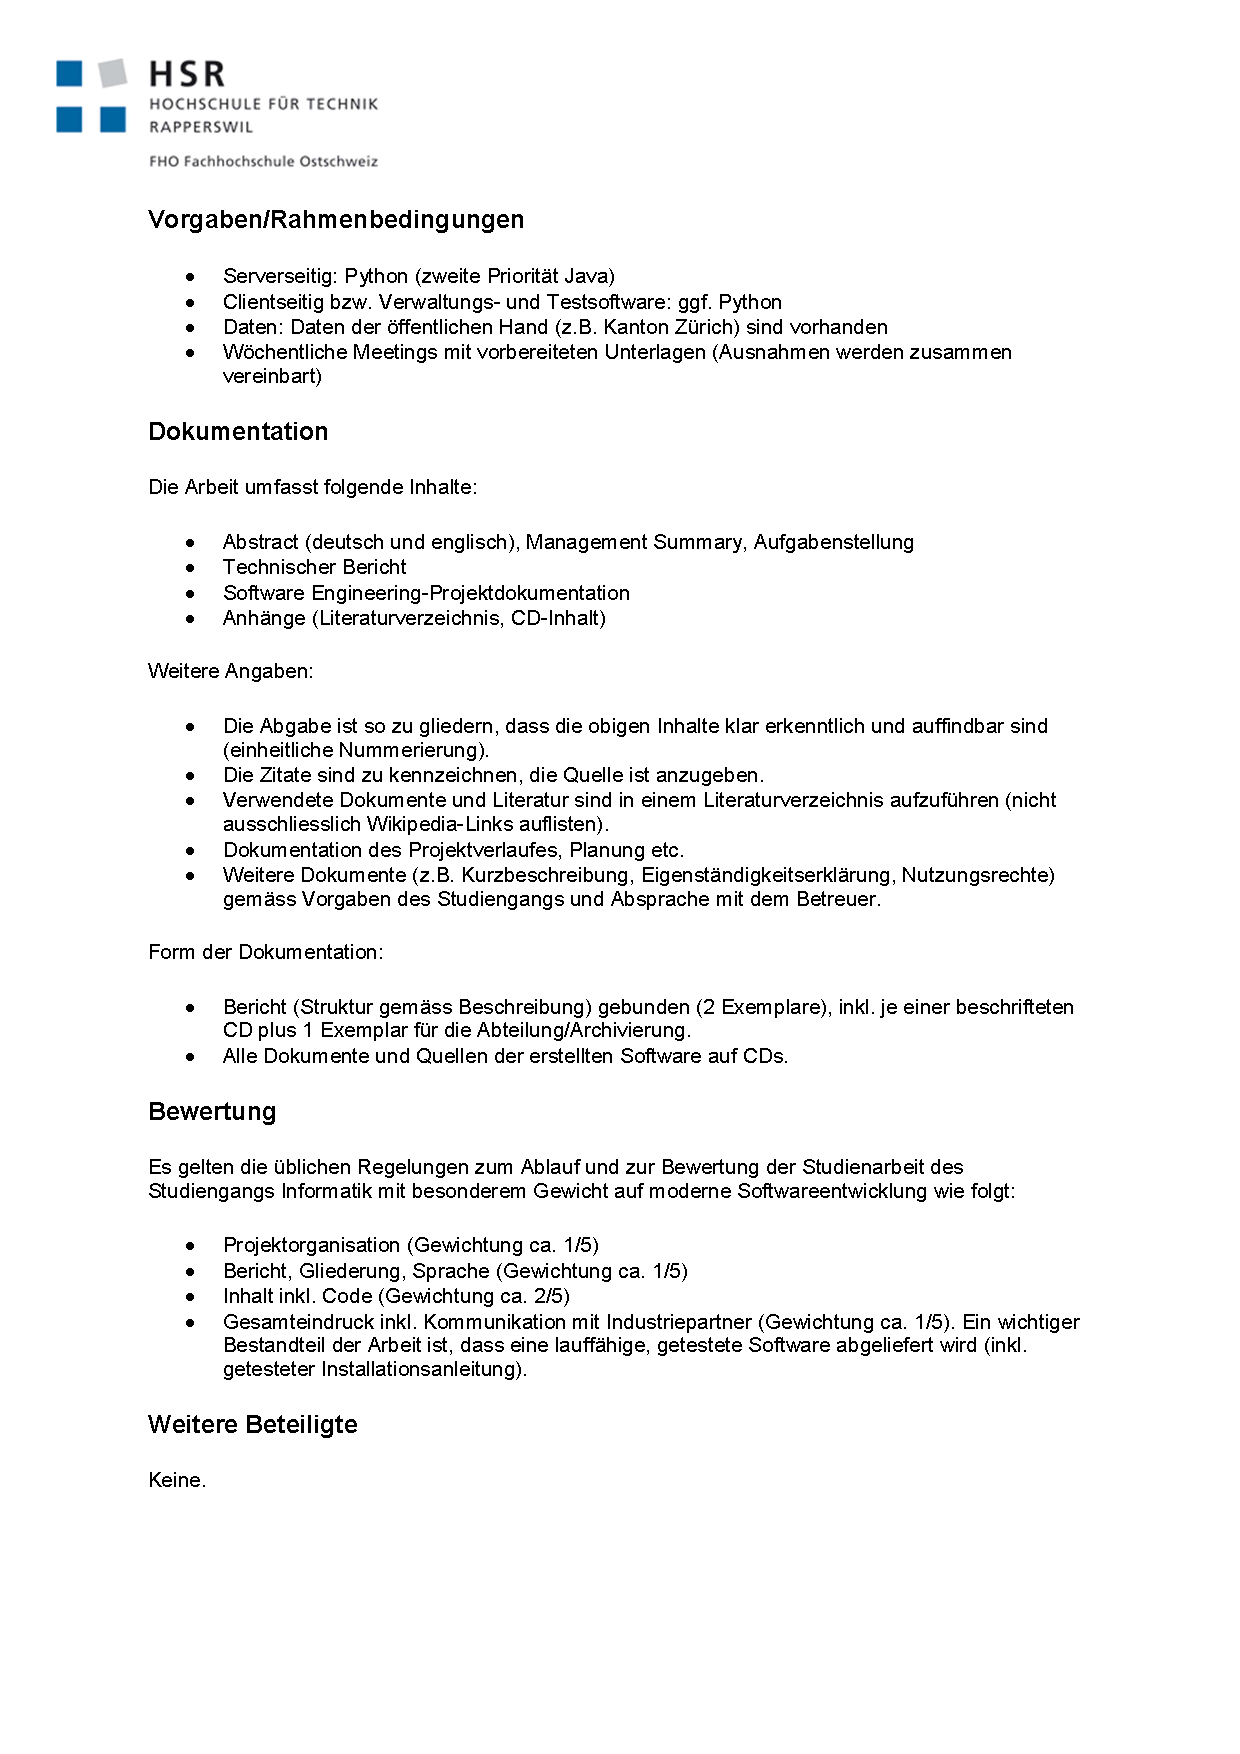
\includepdf[pages=-,offset=75 -75,frame,scale=.75,pagecommand={}]{pdfs/aufgabenstellung2.pdf}

% The main content
%%%%%%%%%%%%%%%%%%
\chapter{Technischer Bericht}
\newpage
\section{Einführung}
\subsection{Vision}
\label{subsec:vision}
\paragraph{Aktuell}
StrongSwan wird standardmässig per Konfigurationsdateien verwaltet, dies zielt stark auf eher versierte Nutzer und Administratoren ab.\\

\paragraph{Vision} 
Es soll eine Applikation entstehen, mit der dieser komplexe Prozess erleichtert wird. Dabei wir auf ein graphisches Interface gesetzt.\\
\section{Stand der Technik}
Android App.

\subsection{Literaturrecherche}
\subsubsection{Suchquellen}
Folgende Quellen wurden uns empfohlen, um Recherchen in diesem Umfeld durchzuführen:
\begin{itemize}
	\item a
    \item b
    \item c
\end{itemize}

\subsubsection{Auswertung}
-

\subsubsection{Fazit}
-
\section{Evaluation Usermanagement}
\subsection{Auswertung}
-

\decision{Evaluation Usermanagement}
-


\section{Evaluation Zertifikatstypen}
\subsection{Auswertung}
-
\decision{Evaluation Zertifikatstypen}
-



\section{Evaluation Zertifikatsbibliothek}
\subsection{Auswertung}
-
\decision{Evaluation Zertifikatsbibliothek}
-
\section{Umsetzungskonzept}
\label{sec:umsetzung}
Die Grundidee für die Umsetzung des Management Tools:
\begin{enumerate}
	\item 1
	\item 2
\end{enumerate}



\newpage
\section{Resultate}
\subsection{Zielerreichung}
-
\subsubsection{Ziel der Aufgabenstellung}
\begin{table}[H]
    \begin{tabular}{|p{6cm}|p{8cm}|}
    \hline    
    \rowcolor{lightblue}
	Ziel & Resultat \\ \hline
	Evaluation eines effizienten Algorithmus zur Erkennung von Fussgängerstreifen auf Orthofotos. & Diverse Algorithmen wurden evaluiert, mit dem Deep Learning Ansatz wurde ein klarer Favorit ermittelt. Mehr dazu unter dem Abschnitt~\ref{sec:suchalgorithmus} auf der Seite~\pageref{sec:suchalgorithmus}.\\ \hline
	Automatische Verarbeitung von Orthofotos. & Es wird automatisch auf Bilder von Bing Maps zugegriffen.\\ \hline
	Extraktion der Koordinaten von Fussgängerstreifen aus Orthofotos (Kanton Zürich, optional Europa oder mehr). & Zürich konnte von der Applikation verarbeitet werden, weiter wurde die Suche auf die Ostschweiz ausgebaut. \\ \hline
	Evaluation des Crowdsourcing-System zur Daten-Validierung und Übertragung in OSM.& Bei der Evaluation des Crowdsourcing-Systems setzte sich MapRoulette durch die Bekanntschaft bei der Community durch. Mehr dazu unter dem Abschnitt~\ref{sec:crowdsourcing} auf der Seite~\pageref{sec:crowdsourcing}. \\ \hline
	Erstellung einer Challenge für das Crowdsourcing-System anhand der gesammelten Daten. & Eine Challenge wurde für MapRoulette generiert und publiziert.\\ \hline
    \end{tabular}
    \caption[Resultate]{Resultate}
\end{table}
Die in der Aufgabenstellung formulierten Ziele konnten alle in einem angemessenem Rahmen erreicht werden. 

\newpage
\subsection{Persönlicher Bericht}
Mit dem Resultat des Projektes sind wir äusserst zufrieden. Es wurde viel neues dazugelernt, sowohl in technischen Bereichen, wie auch in der Teamkommunikation und dem Projektmanagement.
\subsubsection{Neu erlernte Technologien}
\begin{itemize}
	\item Python
	\item \Gls{Docker}
	\item Latex
\end{itemize}
\newpage

\subsection{Dank}
-


\newpage	
\chapter{Software Projektdokumentation}
\newpage 
\section{Einführung}
\subsection{Vision}
\label{subsec:vision}
\paragraph{Aktuell}
StrongSwan wird standardmässig per Konfigurationsdateien verwaltet, dies zielt stark auf eher versierte Nutzer und Administratoren ab.\\

\paragraph{Vision} 
Es soll eine Applikation entstehen, mit der dieser komplexe Prozess erleichtert wird. Dabei wir auf ein graphisches Interface gesetzt.\\
\section{Anforderungsspezifikation}
\subsection{Allgemeine Beschreibung}
Im generellen sind zwei Anwendungsszenarien denkbar:
\begin{itemize}
	\item VPN-Client
	\item VPN-Gateway
\end{itemize}
\medskip
Dabei ist der VPN-Client eine \textbf{Muss}-Anforderung und der VPN-Gateway eine \textbf{Kann}-Anforderung.
\medskip
\subsubsection{VPN-Client}
Die Applikation wird von einem Standard-Nutzer verwendet. Dieser soll VPN Tunnels zu Gateways konfigurieren können und die Tunnels starten und stoppen. Die Konfigurationsmöglichkeiten sind beschränkt, als Richtwert wird der strongSwan Android Client verwendet.\\


\subsubsection{VPN-Gateway}
Der Gateway ist auf Systemadministratoren ausgerichtet. Es soll möglich sein per grafischem Interface strongSwan zu konfigurieren und Tunnels einzurichten, welche als Gateway genutzt werden. 

\subsection{Use Case}
\subsubsection{Aktoren und Stakeholder}
\begin{table}[H]
\centering
    \begin{tabular}{|p{3cm}|p{9cm}|}
    \hline
    \rowcolor{lightblue}
    Aktor & Tätigkeit   \\ \hline
	User  & 
			\begin{itemize}
			\item Konfiguriert VPN-Tunnel als Client
    		\item Startet und stoppt VPN-Tunnel
		\end{itemize}	
	\\ \hline
	Administrator & 
			\begin{itemize}
			\item Konfiguriert VPN-Tunnel als Gateway
    		\item Startet und stoppt VPN-Tunnel
		\end{itemize}	
	\\ \hline
	\end{tabular}
    \caption[Aktoren und Stakeholder]{Aktoren und Stakeholder}
\end{table}

\subsubsection{Use Case Diagramm}
\begin{figure}[H]
\centering
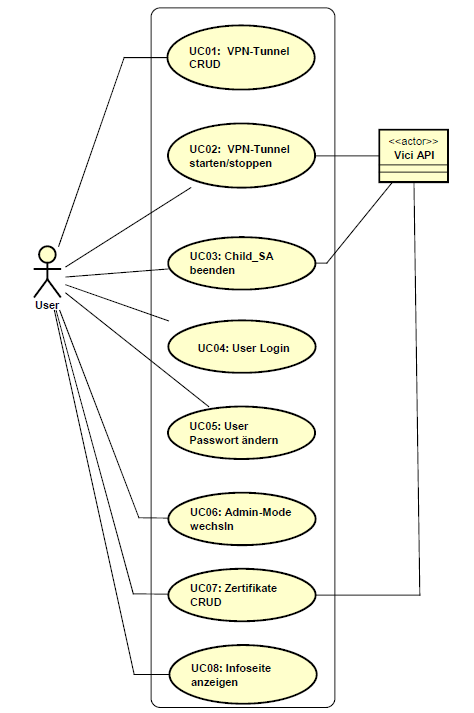
\includegraphics[width=420pt]{images/strongMan_usecase.png}
\caption[Use Case Diagramm]{Use Case Diagramm}
\end{figure}


\subsubsection{Use Cases Brief}
Alle hier definierten Use Cases haben auch ein entsprechendes Mockup im Anhang.
\paragraph{UC01: VPN-Tunnel CRUD}\mbox{} \\
Der User kann einen VPN-Tunnel erfassen / konfigurieren. Dabei hat er eine Auswahl von verschiedenen vordefinierten Tunneltypen. Jeder Tunneltyp hat eigene Konfigurationsfelder, die der User ausfüllen muss. Die Tunnel-Übersichtsseite stellt die Hauptseite der Applikation dar. Dort können die Tunnels bearbeitet und gelöscht werden.

\paragraph{UC02: VPN-Tunnel starten/stoppen}\mbox{} \\
Der User kann einen erfassten VPN-Tunnel starten und stoppen. Dabei wird die Konfiguration über die Vici API geladen. Falls ein VPN-Tunnel nicht aufgebaut werden kann, soll eine passende Fehlermeldung angezeigt werden. 

\paragraph{UC03: Child\_SA beenden}\mbox{} \\
Jeder VPN-Tunnel kann mehrere Child\_SA enthalten. Dieser werden in der Hauptseite angezeigt und können vom User beendet werden. Dieser Use Case interagiert mit der VICI Schnittstelle.

\paragraph{UC04: User Login}\mbox{} \\
Der User loggt sich zu Beginn beim Webseiten Aufruf mit einem Passwort ein. Es existiert dabei nur ein User mit Passwort.

\paragraph{UC05: User Passwort ändern}\mbox{} \\
Sobald der User eingeloggt ist, hat er die Möglichkeit, sein Passwort zu ändern. Dabei gibt er sein altes Passwort einmal und sein neues Passwort zweimal ein.

\paragraph{UC06: Admin-Mode wechseln}\mbox{} \\
Das Userinterface unterscheidet zwischen zwei Modis: User- \& Admin-Mode. Der Mode kann durch einem Klick auf einen Button gewechselt werden. Der Admin-Mode stellt einige Gateway-spezifische Funktionalitäten zusätzlich zur Verfügung, welche der User zur einfacheren Bedienung nicht sieht.

\paragraph{UC07: Zertifikate CRUD}\mbox{} \\
Dem User wird eine Zertifikatsverwaltung zur Verfügung gestellt. Er kann Zertifikate und Private Key's in den gängigen Formaten uploaden, anschauen, updaten (Passwort ändern) und wieder löschen. Die Dateien können mit einem Passwort verschlüsselt sein. Dieser Use Case interagiert unter Umständen mit der VICI Schnittstelle.

\paragraph{UC08: Infoseite anzeigen}\mbox{} \\
Die Infoseite zeigt dem eingeloggten User verschieden Informationen über das installierte System wie Charon Version, installierte Plugins usw.

\subsubsection{Definition Konfigurationsmöglichkeiten UC01}
\paragraph{VPN-Client}\mbox{} \\
Folgende Tunneltypen müssen unterstützt werden:
\begin{itemize}
	\item IKEv2	Zertifikat	
	\item IKEv2 EAP (Benutzername/Passwort)
	\item IKEv2	Zertifikat + EAP (Benutzername/Passwort)
	\item IKEv2	EAP-TLS (Zertifikat)
\end{itemize}

\paragraph{Eingabefelder}
\begin{table}[H]
	\centering
    \begin{tabular}{|p{3cm}|p{7.5cm}|p{6cm}|}
    \hline    
    \rowcolor{lightblue}
	Name & swanclt & vici \\ \hline   
	Profilname & connections.<conn> & <IKE\_SA config name> \\ \hline
	Typ & "Verbindungsarten" & "Verbindungsarten" \\ \hline
	Gateway & connections.<conn>.remote\_addrs & remote-host \\ \hline
	EAP Username & 
connections.<conn>.local<suffix>.eap\_id (Ref: secrets.eap<suffix>.id<suffix>)& <IKE>.remote-eap-id \\ \hline
	EAP Passwort & secrets.eap<suffix>.secret &<secret>.data \\ \hline
	Gateway-Port & connections.<conn>.remote\_port & <IKE>.remote-port \\ \hline
	CA-Zertifikat & connections.<conn>.remote<suffix>.cacerts & \\ \hline
	User-Zertifikat & connections.<conn>.local<suffix>.certs & \\ \hline
	\end{tabular}
    \caption[Eingabefelder VPN-Client]{Eingabefelder VPN-Client}
\end{table}


\paragraph{VPN-Gateway}\mbox{} \\





\newpage
\subsection{Sequenzdiagramm}
\subsubsection{User}
Das Sequenzdiagramm beschreibt...
\newpage
\subsection{Nichtfunktionale Anforderungen}
\subsubsection{Funktionalität}
\paragraph{Sicherheit}
\paragraph{Interoperabilität}
\paragraph{Richtigkeit}
\subsubsection{Zuverlässigkeit}
\paragraph{Wiederherstellbarkeit}
\paragraph{Fehlertoleranz}
\paragraph{Availability}
\subsubsection{Benutzbarkeit}
\paragraph{Robustheit}
\subsubsection{Effizienz}
\subsubsection{Supportability}
\paragraph{Internationalization}


\subsection{Analyse}

\subsubsection{Beschreibung Domain Modell}
-
\section{Implementation}
-
\newpage
\section{Testing}
In der Python Standard Library gibt es das Unit Testing Framework \textbf{unittest}, das es erlaubt Unittests zu implementieren. 
Django's Unit tests basieren auf dieser Library und erweitern diese, beispielsweise erbt \textbf{django.test.TestCase} von \textbf{unittest.TestCase}. Weiter werden auch Integrationtests ermöglicht.

\subsubsection{Beispiel Integrationtests}
\begin{python}
from django.test import Client, TestCase
from django.contrib.auth.models import User

class AboutViewsTests(TestCase):

   def setUp(self):
       self.user = User.objects.create(username='testuser')
       self.user.set_password('12345')
       self.user.save()
       self.client = Client()
       self.client.login(username='testuser', password='12345')

   def test_about_get(self):
       response = self.client.get('/about/')
       self.assertEquals(response.status_code, 200)      
\end{python}

\subsection{Continuous Integration (CI)}
\subsubsection{Anforderungen}
\begin{itemize}
	\item Aufbau von IPsec Tunnel zwischen mindesten zwei Rechnern
	\item automatisierter Ablauf
	\item geringe Einarbeitungszeit in Technologien
	\item möglichst kostenfreie Dienste nutzen
\end{itemize}
\subsubsection{Tools}
\paragraph{GitHub} wird von uns als online Repository verwendet und wird mit dem Versionsverwaltungssystem Git eingesetzt. Weiter bietet es für andere Dienste WebHooks an. 
\paragraph{Travis CI} wird als eigentlicher Continuous Integration Anbieter verwendet, es werden automatisierte Builds und Tests ermöglicht. Travis CI ist für Projekte, welche auf GitHub gehostet werden ausgelegt.

\paragraph{Docker} um Integration Tests zu ermöglichen wird docker-compose eingesetzt, welches gewährleistet mehrere Docker Container zu builden und eine Netzwerk untereinander aufzubauen. \\
\decision{Toolstack CI}
Um einen IPsec Tunnel aufzubauen nutzen wir zwei Docker Container mit Hilfe von docker-compose. Travis CI unterstützt docker-compose und lässt sich nahtlos mit GitHub kombinieren. Diese Technologien sind uns schon bekannt und werden kostenlos zur Verfügung gestellt.

\begin{figure}[H]
\centering
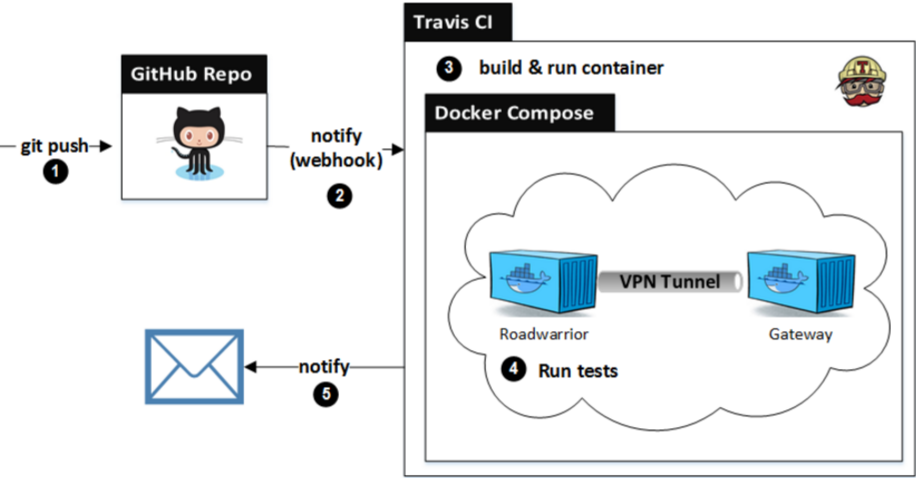
\includegraphics[width=420pt]{images/testing.png}
\caption[Schematische Darstellung der Testumgebung]{Schematische Darstellung der Testumgebung}
\end{figure}
\subsubsection{Ablauf}
\begin{enumerate}
	\item git push, lokaler Code wird auf GitHub publiziert
	\item Travis CI wird durch WebHook notifiziert
	\item Travis CI buildet zwei Docker Container, welche auf der Basis des offiziellen Django Container aufbauen 
	\begin{enumerate}
         \item StrongSwan mit den nötigen Plugins wird installiert und gestartet
         \item Auf dem Roadwarrior wird die strongMan Applikation vom GitHub Repository installiert und der aktuelle Branch wird eingecheckt
      \end{enumerate}
      \item Der Roadwarrior started die Unit- sowie die Integrationstests, dabei werden zwischen den Docker Container diverse Ipsec Tunnels auf- und abgebaut
      \item abschliessend wird über Erfolg oder Misserfolge per Email notifiziert
\end{enumerate}

\newpage
\chapter{Projektmanagement}
\newpage
\section{Rollen und Verantwortlichkeiten}
\subsection{Prof. Keller Stefan}
\begin{figure}[H]
	\centering
	
\includegraphics[width=35mm]{images/asteffen.jpg}
	\caption{Prof. Dr. Andreas Steffen}
\end{figure}
Professor, Institutsleiter ITA

\subsection{Bühler Severin}
\begin{figure}[H]
	\centering
	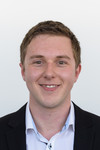
\includegraphics[width=35mm]{images/sbuehler.jpg}
	\caption{Severin Bühler}
\end{figure}
Severin Bühler, Student an der HSR, ist Entwickler des Projektes.
\newpage
\subsection{Kurath Samuel}
\begin{figure}[H]
	\centering
	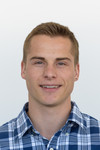
\includegraphics[width=35mm]{images/skurath.jpg}
	\caption{Samuel Kurath}
\end{figure}
Samuel Kurath, Student an der HSR, ist Entwickler des Projektes.

\section{Entwicklungsumgebung und Infrastruktur}
\subsection{IDE (Integrated Development Environment)}
\decision{PyCharm}	
Beiden Projektmitgliedern ist JetBrains Intellij bekannt und \Gls{PyCharm} ist im Umgang nahe zu identisch.
Für Studenten sind die Entwicklungsumgebungen kostenlos verfügbar.
\subsection{SCM (Source Control Management)}
\decision{GitHub}
Der Umgang mit \Gls{Git} ist beiden Projektmitglieder bestens bekannt.
\Gls{GitHub} ist ohne Unkosten von überall verfügbar.
Das Geometalab der HSR publiziert über diesen Weg diverse Projekte.

\subsection{CI (Continuous Integration)}
\decision{CircleCI}
Das finden eines passenden Continuous Integration Tools stellte sich schwieriger dar, als zu Beginn des Projektes erwartet. Während dem SE2 Projekt haben wir Bekanntschaft mit Travis CI gemacht, welches die vielen Abhängigkeiten unseres Codes nicht abdecken konnte. Mit CircleCI fanden wir eine Lösung, die auf Docker Hub zugreifen kann, dann den Build des Images durchführt und schlussendlich die Test durchführt.

\subsection{Projektmanagement Tool}
\decision{Jira}
\Gls{Jira} ist den Projektmitgliedern schon aus dem SE2-Projekt bekannt und hat sich sehr bewährt.
Das Dashboard ist übersichtlich gestaltet. Es ermöglicht eine Übersicht über die aktuellen Tasks auf einen Blick.
Alle Mitglieder haben jederzeit Zugriff auf die Plattform, was die Transparenz erhöht.
Weiter bietet Jira diverse Reports um Auswertungen über das Projekt zu fahren.

\section{Planung}
Am Anfang es Projektes haben wir eine grobe Planung zusammengestellt. Dabei haben wir die Phasen und Meilensteine definiert. Während dem Projekt stellten wir immer wieder grössere oder kleinere Abweichungen an der zu Beginn definierten Planung fest. Dieses ist jedoch nicht erstaunlich, da nie absolut korrekt geplant werden kann. Um solche Schwierigkeiten zu handhaben, erstellten wir ein Risikomanagementdokument.

\subsection{Phasen}
\begin{enumerate}
  \item Inception
  \begin{enumerate}
    \item Aufgabenstellung ausarbeiten
  \end{enumerate}
  \item Elaboration1
  \begin{enumerate}
    \item Evaluation der Algorithmen (Bilderkennung)
  \end{enumerate}
  \item Elaboration2
  \begin{enumerate}
    \item Prototyp 1 (In Orthofotos, Out Koordinaten)
    \item Prototyp 2 MapRoulett
  \end{enumerate}
  \item Construction1
  \begin{enumerate}
    \item Schnittstelle Orthofotos
    \item Optimierungen durch Strassenverlauf und ähnliches
  \end{enumerate}
  \item Construction2
  \begin{enumerate}
    \item MapRoulette (Tags und Quiz)
    \item Koordinaten erfassen	
  \end{enumerate}
  \item Transition
  \begin{enumerate}
    \item Dokumentation abschliessen
    \item Challenge auf Maproulette
  \end{enumerate}
\end{enumerate}
\newpage

\subsection{Meilensteine}
\begin{enumerate}
	\item MS1 Algorithmus für Bilderkennung evaluiert
	\item MS2 Prototyp erstellt
	\item MS3 Automatisierte Datenverarbeitung
	\item MS4 Applikation fertiggestellt
	\item MS5 Challenge auf Maproulette
\end{enumerate}

\subsection{Zeitplanung}
Aufwand: 14 Wochen zu 2 * 16 Stunden = \textbf{448 Stunden}
\begin{tabbing}[H]
    \hspace*{6cm}\=\hspace*{6cm}\= \kill
    Inception \>  1 Woche \\
	Elaboration1 \>	3 Wochen \\
	Elaboration2 \>	4 Wochen \\
	Construction1 \> 3 Wochen \\
	Construction2 \> 1 Wochen \\
	Transition \> 2 Wochen \\
\end{tabbing}



\begin{landscape}
	\begin{figure}[H]
		\centering
		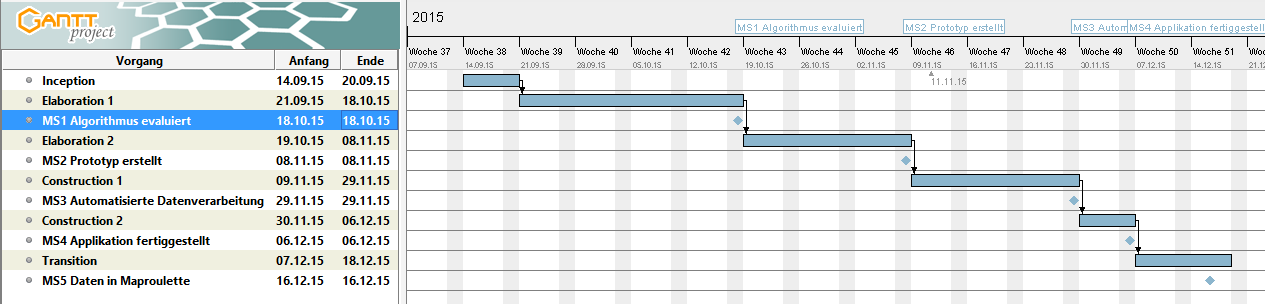
\includegraphics[width=250mm]{images/Gantt.png}
		\caption{Gantt Chart}
	\end{figure}
\section{Risiken}
Um den Problemen, die während des Projekts auftreten können entgegenzuwirken, haben wir eine Risiko Analyse durchgeführt. Diese konnte dann bei der Planung eingesetzt werden.

\subsection{Technische Risiken}
\begin{table}[H]
    \begin{tabular}{|p{0.4cm}|p{1.8cm}|p{7cm}|p{1.5cm}|p{2.25cm}|p{1.75cm}|p{3cm}|p{4cm}|}
    \hline    
    \rowcolor{lightblue}
    Nr & Titel & Beschreibung & maximaler Schaden & Eintrittswahr-scheinlichkeit & Gewichteter Schaden & Vorbeugung & Verhalten beim Eintreten \\ \hline
	R1 & Einarbeitung Python & Python ist den Teammitgliedern teils bekannt, jedoch wurde noch kein grösseres Projekt mit dieser Sprache entwickelt. & 40h & 10\% &4h & Evaluation des Wissensstandes & Informationen bei Studenten einholen, die Python gut kennen \\ \hline
	R2 & Installation OpenCV & Die Installation von OpenCV mit den Contrib Package ist bekanntermassen ein grosse Hürde & 16h & 50\% & 8h & Installation mit Tutorials durchführen & Rücksprache mit Felix Morgner \\ \hline
	R3 & Detektion & Der Algorithmus, der Fussgängerstreifen erkennt, liefert zu schlechte Resultate und kann nicht gebraucht werden. & 40h & 50\% & 20h & Analyse diverser Algorithmen in der Evaluation & Gespräch mit Guido Schuster suchen \\ \hline
	R4 & Download Orthofoto & Download der Orthofotos von Bing oder ähnlichen Quellen ist nicht möglich & 50h & 30\% & 15h & Alternativen im Auge behalten & Auf Bildmaterial der HSR zurückgreifen \\ \hline
	R5 & Software ist zu langsam & Der Download der Orthofotos oder die Detektion kann einige Zeit in Anspruch nehmen.	& 60h & 70\% & 42h & Konzept für Parallelisierung erarbeiten & Fläche einschränken, - Grössere und mehrere Maschinen verwenden. \\ \hline
    \end{tabular}
    \caption[Risiken]{Risiken - Die technischen Risiken wurden zu Beginn des Projektes, wie in der Tabelle ersichtlich, definiert.}
\end{table}
\end{landscape}

\subsection{Auswertung}
\paragraph{R1	Einarbeitung Python}
Risiko ist nicht eingetreten, die Entwickler hatte keine Mühe mit Python zu arbeiten.

\paragraph{R2 Installation OpenCV}
Risiko ist in vollem Umfang eingetreten. Die Installation und Kompilation stellte sich als äusserst Trickreich heraus.

\paragraph{R3 Detektion}
Die Detektion stellte die Hauptaufgabe unserer Arbeit dar, ist jedoch gleichzeitig eine der Risiko reichsten, da Bilderkennung ein nicht ganz triviales Problem ist. Das Implementieren und Testen der verschieden Algorithmen war sehr zeitaufwändig, was dazu führte, dass auch dieses Risiko eingetroffen ist.

\paragraph{R4 Download Orthofoto}
Während des Projektes, wechselten wir mehrmals die API für den Download, was sich auch hier auf einen erhöhten Aufwand auswirkte. 

\paragraph{R5 Software ist zu langsam}
Durch den Einsatz von RQ in Kombination mit Redis wurde diesem Risiko Einhalt geboten. \\

\begin{table}[H]
	\centering
    \begin{tabular}{|p{2cm}|p{5cm}|p{2cm}|}
    \hline    
    \rowcolor{lightblue}
	Nr & Titel & Schaden \\ \hline   
	R1 & Einarbeitung Python & 0h \\ \hline
	R2 & Installation OpenCV & 20h \\ \hline
	R3 & Detektion & 60h \\ \hline
	R4 & Download Orthofoto & 12h \\ \hline
	R5 & Software ist zu langsam & 0h \\ \hline
	\rowcolor{lightblue}
	Total &  & 92h \\ \hline
    \end{tabular}
    \caption[Risikoauswertung]{Risikoauswertung}
\end{table}
\section{Soll-Ist-Zeit-Vergleich}
Während des ganzen Projektes haben wir in Jira vor jeder Phase die jeweiligen Tasks definiert und den Aufwand dazu geschätzt (Soll). Weiter haben wir dann auch die effektive Zeit zu den Tasks erfasst (Ist).
\subsection{Inception}
\begin{tabbing}[H]
    \hspace*{3cm}\=\hspace*{5cm}\=\hspace*{3cm}\=\hspace*{3cm}\= \kill
    Start: \> 14.09.2015 \>	Ende: \> 23.09.2015 \\
\end{tabbing}
\newpage
\subsection{Elaboration1}
\begin{tabbing}[H]
    \hspace*{3cm}\=\hspace*{5cm}\=\hspace*{3cm}\=\hspace*{3cm}\= \kill
    Start: \> 23.09.2015 \> Ende: \> 19.10.2015 \\
\end{tabbing}

\subsection{Elaboration2}
\begin{tabbing}[H]
    \hspace*{3cm}\=\hspace*{5cm}\=\hspace*{3cm}\=\hspace*{3cm}\= \kill
    Start: \> 19.10.2015 \> Ende: \>  04.11.2015 \\
\end{tabbing}

\subsection{Construction1}
\begin{tabbing}[H]
    \hspace*{3cm}\=\hspace*{5cm}\=\hspace*{3cm}\=\hspace*{3cm}\= \kill
    Start: \> 04.11.2015 \>	Ende: \>  25.11.2015 \\
\end{tabbing}

\subsection{Construction2}
\begin{tabbing}[H]
    \hspace*{3cm}\=\hspace*{5cm}\=\hspace*{3cm}\=\hspace*{3cm}\= \kill
    Start: \> 04.11.2015 \>	Ende: \>  11.11.2015 \\
\end{tabbing}

\subsection{Transition}
\begin{tabbing}[H]
    \hspace*{3cm}\=\hspace*{5cm}\=\hspace*{3cm}\=\hspace*{3cm}\= \kill
    Start: \> 11.12.2015 \> Ende: \>  18.12.2015 \\
\end{tabbing}

\subsection{Übersicht}
\begin{table}[H]
\centering
    \begin{tabular}{|p{5cm}|p{2cm}|p{2cm}|p{2cm}|}
    \hline    
    \rowcolor{lightblue}
	Phase & Soll & Ist & Differenz \\ \hline
	Inception & 36.00 &	45.50 &	9.50 \\ \hline
	Elaboration1 & 111.00 & 150.50	& 39.50 \\ \hline
	Elaboration2 & 98.00 & 105.75 & 7.75 \\ \hline
	Construction1 & 110.00 & 122.50 & 12.50 \\ \hline
	Construction1 & 58.00 & 88.50 & 30.50 \\ \hline
	Transition & 34.00 & 52.00 & 18.00 \\ \hline
	\rowcolor{lightblue}
	Total & 447.00 & 564.75 & 117.75 \\ \hline
    \end{tabular}
    \caption[Phasen]{Phasen}
\end{table}
\medskip
Schätzen ist wie bekannt, ein relativ schwierige Angelegenheit. So haben wir den Aufwand für die jeweiligen Tasks meist zu tief eingestuft. Stark ins Gewicht fiel die Evaluation und Implementierung des Bilderkennungsalgorithmus.

\newpage
\section{Codestatistik}
\subsection{Test Coverage}
Test Coverage wurde mit dem Tool \textbf{nose} durchgeführt. \\

\begin{table}[H]
\centering
    \begin{tabular}{|l|l|}
    \hline    
    \rowcolor{lightblue}
	Datei & Coverage [\%] \\ \hline
	src/base/Bbox.py & 85 \\ \hline    
	src/base/Node.py & 97 \\ \hline   
	src/base/Street.py & 92 \\ \hline  
	src/base/Tile.py & 98 \\ \hline   
	src/base/TileDrawer.py & 24 \\ \hline  
	src/data/MapquestApi.py & 100 \\ \hline   
	src/data/MultiLoader.py & 94 \\ \hline   
	src/data/StreetLoader.py & 100 \\ \hline   
	src/data/TileLoader.py & 100 \\ \hline   
	src/detection/BoxWalker.py & 100 \\ \hline   
	src/detection/NodeMerger.py & 89 \\ \hline  
	src/detection/StreetWalker.py & 100 \\ \hline   
	src/detection/deep/Convnet.py & 97 \\ \hline   
	src/detection/deep/training/Crosswalk\_dataset.py & 100 \\ \hline  
	src/detection/deep/training.py & 100 \\ \hline   
	src/role/Manager.py & 91 \\ \hline  
	src/role/WorkerFunctions.py & 70 \\ \hline
	\rowcolor{lightblue}
	Durchschnitt &   90.5 \\ \hline
    \end{tabular}
    \caption[Test Coverage]{Test Coverage}
\end{table}

\subsection{Codezeilen}
Die Codezeilen wurden mit Hilfe von \textbf{CLOC} \cite{CLOC} ausgezählt. \\

\begin{table}[H]
\centering
    \begin{tabular}{|p{3cm} |p{3cm} |p{3cm} |}
    \hline    
    \rowcolor{lightblue}
	Sprache & Dateien & Zeilen  \\ \hline   
	Python & 43 & 2045 \\ \hline
    \end{tabular}
    \caption[Codezeilen]{Codezeilen}
\end{table}


\section{Rational Unified Process (RUP)}


Das Projekt Extraction of Crosswalks from Aerial Images führten wir mit dem Vorgehensmodell RUP \cite{RUP} aus.
Dies ist eine iterative Art um Softwareprojekt anzugehen. RUP kennt die Phasen:

\begin{itemize}
	\item Inception, Elaboration, Construction, Transition
\end{itemize}

Um eine feinere Aufteilung zu haben, unterteilten wir die Elaboration, sowie die Construction in je zwei Hälften. 

\subsubsection{Fazit}
Wir hatten Mühe unserem Projekt ein RUP Stempel auf zu drücken, da wir bei der Evaluation der Algorithmen immer wieder grosse Teile unserer Lösung überdenken und auf den Kopf stellen mussten. Es wurde viel geschriebener Code wieder über den Haufen geworfen. Weiter war es schwierig den Phasen gerecht zu werden, nur mit vielen Überstunden konnte am Ende der Elaboration ein Prototyp präsentiert werden, der ein angemessenes Resultat lieferte. Im Nachhinein hätte sich ein agilieres Vorgehensmodell wie Scrum oder ähnlich vielleicht besser bewährt.
 



\newpage
\chapter{Softwaredokumentation}
\newpage
\section{Installation}
\subsection{Redis}
\label{subsec:redis}
Die Installation wurde auf einem Ubuntu Server durchgeführt, welcher das Paketverwaltungssystem Advanced Packaging Tool (APT) verwendet. Die im Anschluss aufgeführten Befehle werden in einer Shell ausgeführt.
Falls Probleme auftreten, bietet Redis ein Quick Start Dokumentation an.

\subsubsection{Installaiton}
\begin{lstlisting}[style=BashInputStyle]
	# sudo apt-get install redis-server
\end{lstlisting}

\subsubsection{Konfiguration}
\begin{lstlisting}[style=BashInputStyle]
	# redis-cli -p 40001
	# CONFIG SET requirepass "crosswalks"
	# redis-cli AUTH crosswalks
\end{lstlisting}

\subsubsection{Starten}
\begin{lstlisting}[style=BashInputStyle]
	# redis-server --port 40001
\end{lstlisting}

\subsection{Keras}
Keras ist die Bibliothek, mit der das neuronale Netz betrieben wird. Die Installation hier muss nur durchgeführt werden, um das Projekt weiterzuentwickeln.

Info: Der Stand von Keras, der wir während dieser Arbeit verwendet haben, ist auf der CD zu finden.
\subsubsection{Installation Theano}
\begin{lstlisting}[style=BashInputStyle]
	# apt-get update
	# apt-get install -y git libopenblas-dev python-dev python-pip 
	python-nose python-numpy python-scipy
	# pip install git+git://github.com/Theano/Theano.git
\end{lstlisting}
\subsubsection{Installation Keras}
\begin{lstlisting}[style=BashInputStyle]
	# apt-get install -y libhdf5-dev python-h5py python-yaml
	# pip install --upgrade six
	# cd /root
	# git clone https://github.com/fchollet/keras.git 
	# cd keras
	# python setup.py install
\end{lstlisting}
\newpage

\subsection{Docker}
\label{subsec:docker}
Die Installation unserer Applikation beinhaltet diverse Abhängigkeiten, welche für die Installation einerseits viel Zeit in Anspruch nehmen und anderseits auch nicht wirklich trivial sind.. \\
\decision{Docker}
Deshalb haben wir ein Docker Image ersellt, das auf Dockerhub \cite{DokerCrosswalk} frei zur Verfügung gestellt wird und somit den DevOps Prozess massiv vereinfach.\\

\subsubsection{Installation}
Bei der Installation von Docker ist zu beachten, dass die Anwendung nur auf 64-Bit Maschinen läuft. Weiter wurden die nachfolgenden Befehle auf Ubuntu durchgeführt und variieren deshalb je nach Betriebssystemen. 

\paragraph{Vorarbeit}
\begin{lstlisting}[style=BashInputStyle]
	# sudo apt-key adv --keyserver hkp://p80.pool.sks
	-keyservers.net:80 --recv-		
	keys 58118E89F3A912897C070ADBF76221572C52609D
	# echo 'deb https://apt.dockerproject.org/repo ubuntu-precise main' 
	>> /etc/apt/sources.list.d/docker.list
	# apt-get update
	# apt-cache policy docker-engine
	# sudo apt-get install linux-image-extra-$(uname -r)
\end{lstlisting}
\paragraph{Docker installieren}
\begin{lstlisting}[style=BashInputStyle]
	# sudo apt-get install docker-engine
\end{lstlisting}

\subsubsection{Starten}
\begin{lstlisting}[style=BashInputStyle]
	# sudo service docker start
	# sudo docker run hello-world
\end{lstlisting}


\section{Benutzerhandbuch}
\subsection{Suche der Fussgängerstreifen}
Um die Suche der Fussgängerstreifen durchzuführen, muss eine Redis Datenbank zur Verfügung stehen. Weiter muss auf den Rechnern, die als Jobworker tätig sind, Docker installiert sein. \\
Die Installationen sind in folgenden Abschnitten aufgeführt:
\begin{itemize}
	\item Redis:  Abschnitt~\ref{subsec:redis} auf der Seite~\pageref{subsec:redis}
	\item Docker: Abschnitt~\ref{subsec:docker} auf der Seite~\pageref{subsec:docker}
\end{itemize}

\subsubsection{Einführung}
Wir haben unsere Applikation in drei Rollen aufgeteilt:
\begin{itemize}
	\item Manager
	\begin{itemize}
		\item Unterteilt eine grosse Bounding Box in kleinere Boxen mit einer Höhe und Breite von jeweils 2 Kilometern und stellt dies als Jobs in die Queue.
	\end{itemize}
	\item Jobworker
	\begin{itemize}
		\item Arbeite die Jobs der Queue ab.
		\item Gefundene Fussgängerstreifen , welche noch nicht in OpenSteetMap erfasst sind, werden als Job Resultat in die Queue gestellt.
	\end{itemize}
	\item Resultworker
	\begin{itemize}
		\item Schlussendlich werden die Resultate zusammen getragen und in ein JSON File geschrieben.
	\end{itemize}
\end{itemize}

Dieser Ablauf ist genauer beschrieben unter dem Abschnitt~\ref{subsec:ablauf} auf der Seite~\pageref{subsec:ablauf}

\newpage
\subsubsection{Anwendung}
Dank Docker kann unsere Applikation innert Minuten gestartet werden.

\paragraph{Docker Pull}\mbox{}\\
\begin{lstlisting}[style=BashInputStyle]
	# docker pull murthy10/osm-crosswalk-detection
\end{lstlisting}

\paragraph{Manager}\mbox{}\\
\begin{lstlisting}[style=BashInputStyle]
	# docker run murthy10/osm-crosswalk-detection REDIS_IP_ADDR 
 	--role manager left bottom right top
\end{lstlisting}
Left, Bottom, Right, Top entsprechen den Koordinaten im WGS84 Format. \\
Ostschweiz: left=8.361002, bottom=47.166994, right=8.977610, top=47.706676

\paragraph{Jobworker}\mbox{}\\
\begin{lstlisting}[style=BashInputStyle]
	# docker run murthy10/osm-crosswalk-detection REDIS_IP_ADDR 
 	--role jobworker
\end{lstlisting}
Jobworker können auf beliebig vielen Rechnern gestartet werden.\\

\paragraph{Resultworker}\mbox{}\\
\begin{lstlisting}[style=BashInputStyle]
	# docker run murthy10/osm-crosswalk-detection REDIS_IP_ADDR 
 	--role resultworker
\end{lstlisting}
Die Resultate werden in der Datei crosswalks.json gespeichert. Diese findet man im Verzeichnis in dem der Resultworker gestartet wurde.

\subsubsection{Struktur JSON}
Die Struktur der crosswalks.json Datei ist folgendermassen aufgebaut:
\medskip
\begin{python}
{
	"crosswalks": 
	[
		{"latitude": 47.0, "longitude": 8.3},
		{"latitude": 48.0, "longitude": 8.4}
	]
}
\end{python}

\newpage

\subsection{Daten visualisieren}
Um das Resultat des Erkennungsalgorithmus zu visualisieren bot sich das Tool CartoDB \cite{CartoDB} an. Dieses ermöglicht Daten in diversen Formaten hochzuladen und auf einer Karte anzuzeigen.

\subsubsection{Vorgehen}
\begin{enumerate}
	\item Daten (crosswalk.json) mit den Spalten latitude und longitude. in CSV Format umwandeln
	\item CSV Datei in CartoDB als neues Dataset hochladen.
\end{enumerate}

\subsubsection{Struktur CSV}
Die Struktur der CSV Datei gliedert sich wie folgt:
\medskip
\begin{python}
	latitude,	longitude
	47.0,		8.3
	48.0,		8.4
\end{python}


\subsubsection{Daten selektieren}
CartoDB ermöglicht eine Selektion der Daten. So kann zum Beispiel ein Polygon selektiert werden.
\medskip
\begin{python}
SELECT * FROM dataset WHERE ST_WITHIN(
 	ST_Transform(the_geom, 4326), ST_SetSRID(
 	ST_GeomFromGeoJSON('{ "type": "Polygon",
        "coordinates": [
          [ [8.81429672241211,
             47.22971054221563],
            [8.8385009765625,
             47.22877798599878],
            [8.820991516113281,
             47.2185187846731],
            [8.81429672241211,
             47.22971054221563]
          ]
        ] }'), 
   4326)) 
\end{python}
\newpage
\subsection{Challenge erstellen}
Nach dem die Fussgängerstreifen detektiert wurden und die Datei crosswalks.json erstellt wurde, muss dies noch in ein passendes Format für MapRoulette gebracht werden. Dazu haben wir ein Python Skript geschrieben, welches aus jedem gefundenen Fussgängerstreifen einen Task generiert.

\subsubsection{Anwendung}
Für eine Challenge benötigt es die Datei challange.json, welches die Challenge beschreibt und ein zweite Datei tasks.json, in dem sich die Tasks befinden.\\

\paragraph{Tasks generieren}\mbox{}\\
\begin{lstlisting}[style=BashInputStyle]
 # python TaskGenerator.py crosswalks.json
\end{lstlisting}

\paragraph{Challenge publizieren}\mbox{}\\
\begin{lstlisting}[style=BashInputStyle]
 # curl -u devuser:mylittlesony -vX 
   POST http://maproulette.org/api/admin/challenge/
   crosswalk-detection/tasks -d @tasks.json 
   --header "Content-Type: application:json"
\end{lstlisting}

\paragraph{Tasks publizieren}\mbox{}\\
\begin{lstlisting}[style=BashInputStyle]
 # curl -u devuser:mylittlesony -vX 
   POST http://maproulette.org/api/admin/challenge/
   crosswalk-detection -d @challenge.json 
   --header "Content-Type: application:json"
\end{lstlisting}


Als Hilfestellung zum Erstellen von MapRoulette Challanges gibt es ein empfehlenswertes Tutorial \cite{Tutorial}.

\newpage
\subsection{Keras Training}
Für das Training des Neuronalen Netzes steht ein eigenes Docker Image \cite{DokerKeras} auf Docker Hub bereit. Das Image basiert auf einem offiziellen Nvidia Cuda Image und ist fähig mit einer Nvidia Grafikkarte zu arbeiten. Die Grafikkarte wird mit Hilfe des nvidia-docker Projekts geladen. CUDA muss dabei auf dem Host Rechner installiert sein.


\subsubsection{Keras Image}
\paragraph{Download des nvidia-docker Projekts}\mbox{}\\
\begin{lstlisting}[style=BashInputStyle]
	# git clone https://github.com/NVIDIA/nvidia-docker.git
	# cd nvidia-docker
\end{lstlisting}

\paragraph{Herunterladen des Images}\mbox{}\\
\begin{lstlisting}[style=BashInputStyle]
	# docker pull sebu/keras_cuda
\end{lstlisting}	

\paragraph{Start des Containers und mount der Grafikkarte Nummer 0}\mbox{}\\
\begin{lstlisting}[style=BashInputStyle]
	#GPU=0 ./nvidia-docker run -i -t sebu/keras_cuda /bin/bash
\end{lstlisting}

Achtung: Die Keras Bibliothek entwickelt sich ständig weiter. Auch die Interfaces der populärsten Klassen können sich ändern und haben sich auch schon während diesem Projekt verändert! In diesem Keras Docker Image ist der Stand von Keras installiert, mit dem wir gearbeitet haben. Keras bietet leider keine Versionierung an. Der von uns verwendete Stand ist auch auf der mitglieferten CD erhältlich.

Ein Beispiel für das Training eines Neuronalen Netzes kann in examples/ConvnetTrainer.py und in den Keras eigenen Examples eingesehen werden.

\newpage
\appendix
\newpage
\newpage
\chapter{Inhalt der CD}
Der Inhalt der CD glieder sich folgendermassen:
\begin{figure}[H]
\dirtree{%
.1 CD.
.2 Studienarbeit.pdf.
.2 0\_AUFGABE.
.3 Original Aufgabenstellung.
.2 1\_CODE.
.3 GitHub Repository.
.2 2\_DOKUMENTATION.
.3 Protokolle.
.3 Poster.
.2 3\_RESULTAT.
.3 Geodaten.
.2 4\_ANHANG.
.3 Keras.
}
\end{figure}
\newpage

\chapter{Eigenständigkeitserklärung}

Wir erklären hiermit,
\begin{itemize}
	\item dass wir die vorliegende Arbeit selber und ohne fremde Hilfe durchgeführt haben, ausser derjenigen, welche explizit in der Aufgabenstellung erwähnt sind oder mit dem Betreuer schriftlich vereinbart wurden.
	\item dass wir sämtliche verwendeten Quellen erwähnt und gemäss gängigen wissenschaftlichen Zitierregeln korrekt angegeben haben.
	\item dass wir keine durch Copyright geschützten Materialien (z.B. Bilder) in dieser Arbeit in unerlaubter Weise genutzt haben.
\end{itemize}

\vspace{2cm}

Ort, Datum:

\begin{itemize}
	\item[] Rapperswil, \today
\end{itemize}


\vspace{1cm}
Namen, Unterschriften:
\vspace{2cm}
\begin{tabbing}[H]
    \hspace*{1cm}\=\hspace*{8cm}\=\hspace*{6cm}\= \kill
     \> Severin Bühler \> Samuel Kurath \\
\end{tabbing}

\begingroup     
\let\clearpage\relax        
\printglossary[title=\chapter{Glossar}]
\endgroup
% Bibliography
%%%%%%%%%%%%%%
\bibliographystyle {alpha}
\bibliography{index/bibliography}

\end{document}


\newpage
